\documentclass[twoside]{book}

% Packages required by doxygen
\usepackage{fixltx2e}
\usepackage{calc}
\usepackage{doxygen}
\usepackage[export]{adjustbox} % also loads graphicx
\usepackage{graphicx}
\usepackage[utf8]{inputenc}
\usepackage{makeidx}
\usepackage{multicol}
\usepackage{multirow}
\PassOptionsToPackage{warn}{textcomp}
\usepackage{textcomp}
\usepackage[nointegrals]{wasysym}
\usepackage[table]{xcolor}

% Font selection
\usepackage[T1]{fontenc}
\usepackage[scaled=.90]{helvet}
\usepackage{courier}
\usepackage{amssymb}
\usepackage{sectsty}
\renewcommand{\familydefault}{\sfdefault}
\allsectionsfont{%
  \fontseries{bc}\selectfont%
  \color{darkgray}%
}
\renewcommand{\DoxyLabelFont}{%
  \fontseries{bc}\selectfont%
  \color{darkgray}%
}
\newcommand{\+}{\discretionary{\mbox{\scriptsize$\hookleftarrow$}}{}{}}

% Page & text layout
\usepackage{geometry}
\geometry{%
  a4paper,%
  top=2.5cm,%
  bottom=2.5cm,%
  left=2.5cm,%
  right=2.5cm%
}
\tolerance=750
\hfuzz=15pt
\hbadness=750
\setlength{\emergencystretch}{15pt}
\setlength{\parindent}{0cm}
\setlength{\parskip}{3ex plus 2ex minus 2ex}
\makeatletter
\renewcommand{\paragraph}{%
  \@startsection{paragraph}{4}{0ex}{-1.0ex}{1.0ex}{%
    \normalfont\normalsize\bfseries\SS@parafont%
  }%
}
\renewcommand{\subparagraph}{%
  \@startsection{subparagraph}{5}{0ex}{-1.0ex}{1.0ex}{%
    \normalfont\normalsize\bfseries\SS@subparafont%
  }%
}
\makeatother

% Headers & footers
\usepackage{fancyhdr}
\pagestyle{fancyplain}
\fancyhead[LE]{\fancyplain{}{\bfseries\thepage}}
\fancyhead[CE]{\fancyplain{}{}}
\fancyhead[RE]{\fancyplain{}{\bfseries\leftmark}}
\fancyhead[LO]{\fancyplain{}{\bfseries\rightmark}}
\fancyhead[CO]{\fancyplain{}{}}
\fancyhead[RO]{\fancyplain{}{\bfseries\thepage}}
\fancyfoot[LE]{\fancyplain{}{}}
\fancyfoot[CE]{\fancyplain{}{}}
\fancyfoot[RE]{\fancyplain{}{\bfseries\scriptsize Generated by Doxygen }}
\fancyfoot[LO]{\fancyplain{}{\bfseries\scriptsize Generated by Doxygen }}
\fancyfoot[CO]{\fancyplain{}{}}
\fancyfoot[RO]{\fancyplain{}{}}
\renewcommand{\footrulewidth}{0.4pt}
\renewcommand{\chaptermark}[1]{%
  \markboth{#1}{}%
}
\renewcommand{\sectionmark}[1]{%
  \markright{\thesection\ #1}%
}

% Indices & bibliography
\usepackage{natbib}
\usepackage[titles]{tocloft}
\setcounter{tocdepth}{3}
\setcounter{secnumdepth}{5}
\makeindex

% Hyperlinks (required, but should be loaded last)
\usepackage{ifpdf}
\ifpdf
  \usepackage[pdftex,pagebackref=true]{hyperref}
\else
  \usepackage[ps2pdf,pagebackref=true]{hyperref}
\fi
\hypersetup{%
  colorlinks=true,%
  linkcolor=blue,%
  citecolor=blue,%
  unicode%
}

% Custom commands
\newcommand{\clearemptydoublepage}{%
  \newpage{\pagestyle{empty}\cleardoublepage}%
}

\usepackage{caption}
\captionsetup{labelsep=space,justification=centering,font={bf},singlelinecheck=off,skip=4pt,position=top}

%===== C O N T E N T S =====

\begin{document}

% Titlepage & ToC
\hypersetup{pageanchor=false,
             bookmarksnumbered=true,
             pdfencoding=unicode
            }
\pagenumbering{roman}
\begin{titlepage}
\vspace*{7cm}
\begin{center}%
{\Large Emmeth }\\
\vspace*{1cm}
{\large Generated by Doxygen 1.8.11}\\
\end{center}
\end{titlepage}
\clearemptydoublepage
\tableofcontents
\clearemptydoublepage
\pagenumbering{arabic}
\hypersetup{pageanchor=true}

%--- Begin generated contents ---
\chapter{R\+E\+A\+D\+ME}
\label{md_README}
\hypertarget{md_README}{}
\input{md_README}
\chapter{T\+O\+DO}
\label{md_TODO}
\hypertarget{md_TODO}{}

\begin{DoxyItemize}
\item Include poppler or another pdf library
\item Add the bookstore 
\end{DoxyItemize}
\chapter{Description how to handle the X\+ML Files}
\label{md_XMLHandlers}
\hypertarget{md_XMLHandlers}{}
\subsection*{How it works}

Reads the xml file in a specific way to display it. Every xml file needs to be based on a specific validation file (xsd). It need to have the filename based on the xml schema. The xml syntax is read through a

Eg.\+: Tanach-\/xml has various book files. The folder for the xml files needs to have the same name as the schema. (tanach-\/xml). Tanach-\/xml needs a validation file in xsd format (tanach-\/xml.\+xsd). To check if the file in the folder is an actual tanach-\/xml file or something else. Tanach-\/xml needs a json file with the same schema name (tanach-\/xml.\+json), to read an process the content correctly.

Folder\+: xml -\/$>$ validation file -\/$>$ json -\/$>$precessing.

\subsection*{Structure of the json file}

Xml-\/tag \+: operation

\subsection*{Operations}

Usage on how to handle the X\+ML tags.


\begin{DoxyItemize}
\item ignore -\/ ignores the tag.
\item important
\item read -\/ simply reads the tag and displays the content/children in the X\+M\+L\+Reader.
\item desc -\/ reads the content and displays it in the File Description.
\item encoding -\/ important for the file encoding.
\item abbrev -\/ is used for the book abbreviation (searchable).
\item chapter -\/ displays the whole chapter.
\item word -\/ the simple word to display.
\item verse -\/ displays the whole verse.
\item value -\/ a numerical value (usally an attribute).
\item attrib -\/ a simple attribute (usally text).
\item link -\/ U\+RL link.
\item folder -\/ all the necessary books are in a folder.
\item single -\/ all the necessary books are in the same file. 
\end{DoxyItemize}
\chapter{Hierarchical Index}
\section{Class Hierarchy}
This inheritance list is sorted roughly, but not completely, alphabetically\+:\begin{DoxyCompactList}
\item \contentsline{section}{htmlreader}{\pageref{classhtmlreader}}{}
\item \contentsline{section}{json\+Parser}{\pageref{classjson_parser}}{}
\item \contentsline{section}{Libary}{\pageref{class_libary}}{}
\item \contentsline{section}{pdf\+Reader}{\pageref{classpdf_reader}}{}
\item Q\+Dialog\begin{DoxyCompactList}
\item \contentsline{section}{login\+Dialog}{\pageref{classlogin_dialog}}{}
\item \contentsline{section}{settingsdialog}{\pageref{classsettingsdialog}}{}
\end{DoxyCompactList}
\item Q\+Main\+Window\begin{DoxyCompactList}
\item \contentsline{section}{Main\+Window}{\pageref{class_main_window}}{}
\end{DoxyCompactList}
\item Q\+Widget\begin{DoxyCompactList}
\item \contentsline{section}{about\+Dialog}{\pageref{classabout_dialog}}{}
\item \contentsline{section}{bookstore}{\pageref{classbookstore}}{}
\end{DoxyCompactList}
\item \contentsline{section}{txteditor}{\pageref{classtxteditor}}{}
\item \contentsline{section}{xml\+Reader}{\pageref{classxml_reader}}{}
\end{DoxyCompactList}

\chapter{Class Index}
\section{Class List}
Here are the classes, structs, unions and interfaces with brief descriptions\+:\begin{DoxyCompactList}
\item\contentsline{section}{\hyperlink{classabout_dialog}{about\+Dialog} }{\pageref{classabout_dialog}}{}
\item\contentsline{section}{\hyperlink{classbookstore}{bookstore} }{\pageref{classbookstore}}{}
\item\contentsline{section}{\hyperlink{classhtmlreader}{htmlreader} }{\pageref{classhtmlreader}}{}
\item\contentsline{section}{\hyperlink{classjson_parser}{json\+Parser} }{\pageref{classjson_parser}}{}
\item\contentsline{section}{\hyperlink{class_libary}{Libary} }{\pageref{class_libary}}{}
\item\contentsline{section}{\hyperlink{classlogin_dialog}{login\+Dialog} }{\pageref{classlogin_dialog}}{}
\item\contentsline{section}{\hyperlink{class_main_window}{Main\+Window} }{\pageref{class_main_window}}{}
\item\contentsline{section}{\hyperlink{classpdf_reader}{pdf\+Reader} }{\pageref{classpdf_reader}}{}
\item\contentsline{section}{\hyperlink{classsettingsdialog}{settingsdialog} }{\pageref{classsettingsdialog}}{}
\item\contentsline{section}{\hyperlink{classtxteditor}{txteditor} }{\pageref{classtxteditor}}{}
\item\contentsline{section}{\hyperlink{classxml_reader}{xml\+Reader} }{\pageref{classxml_reader}}{}
\end{DoxyCompactList}

\chapter{Class Documentation}
\hypertarget{classabout_dialog}{}\section{about\+Dialog Class Reference}
\label{classabout_dialog}\index{about\+Dialog@{about\+Dialog}}
Inheritance diagram for about\+Dialog\+:\begin{figure}[H]
\begin{center}
\leavevmode
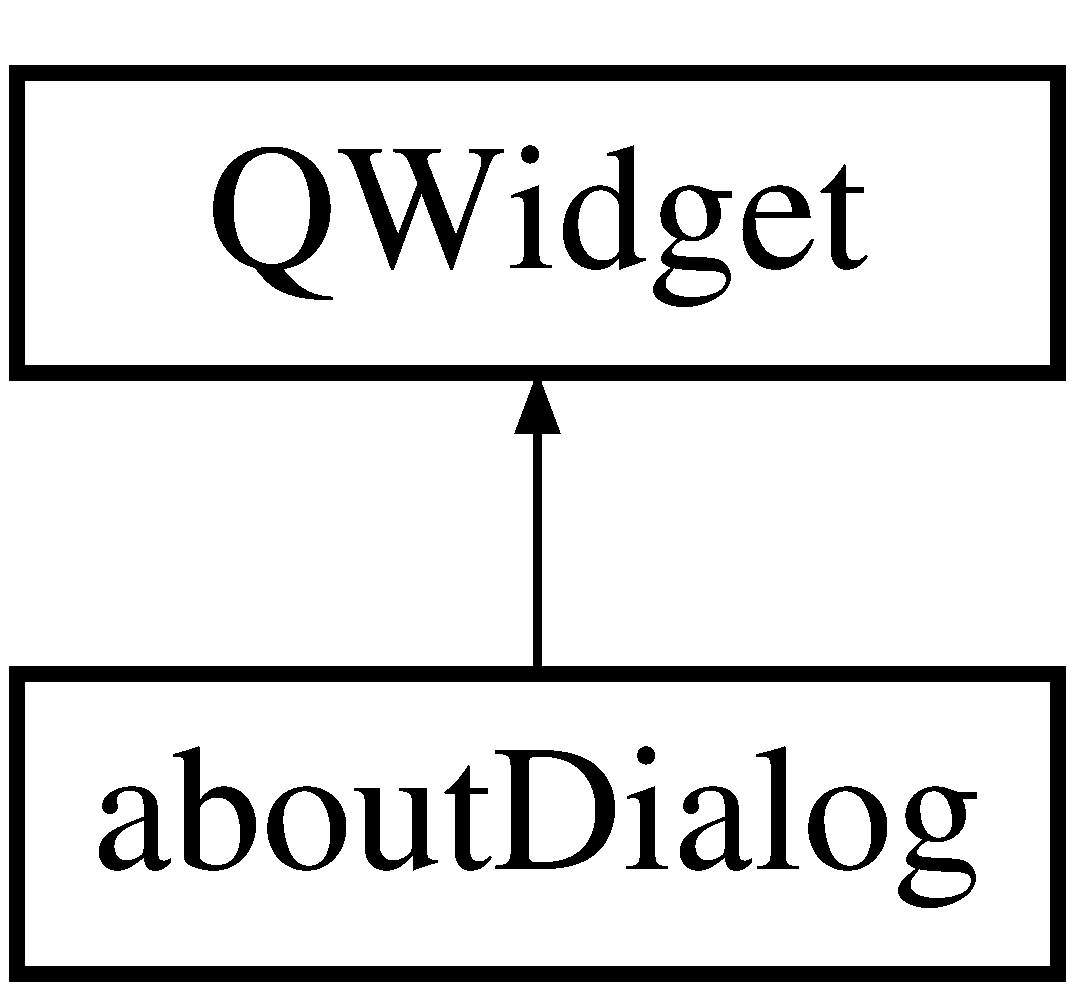
\includegraphics[height=2.000000cm]{classabout_dialog}
\end{center}
\end{figure}
\subsection*{Static Public Member Functions}
\begin{DoxyCompactItemize}
\item 
static void {\bfseries open} ()\hypertarget{classabout_dialog_a7be2b15dd84e22bcf4373fa89182c344}{}\label{classabout_dialog_a7be2b15dd84e22bcf4373fa89182c344}

\end{DoxyCompactItemize}


The documentation for this class was generated from the following files\+:\begin{DoxyCompactItemize}
\item 
about\+Dialog.\+h\item 
about\+Dialog.\+cpp\end{DoxyCompactItemize}

\hypertarget{classbookstore}{}\section{bookstore Class Reference}
\label{classbookstore}\index{bookstore@{bookstore}}
Inheritance diagram for bookstore\+:\begin{figure}[H]
\begin{center}
\leavevmode
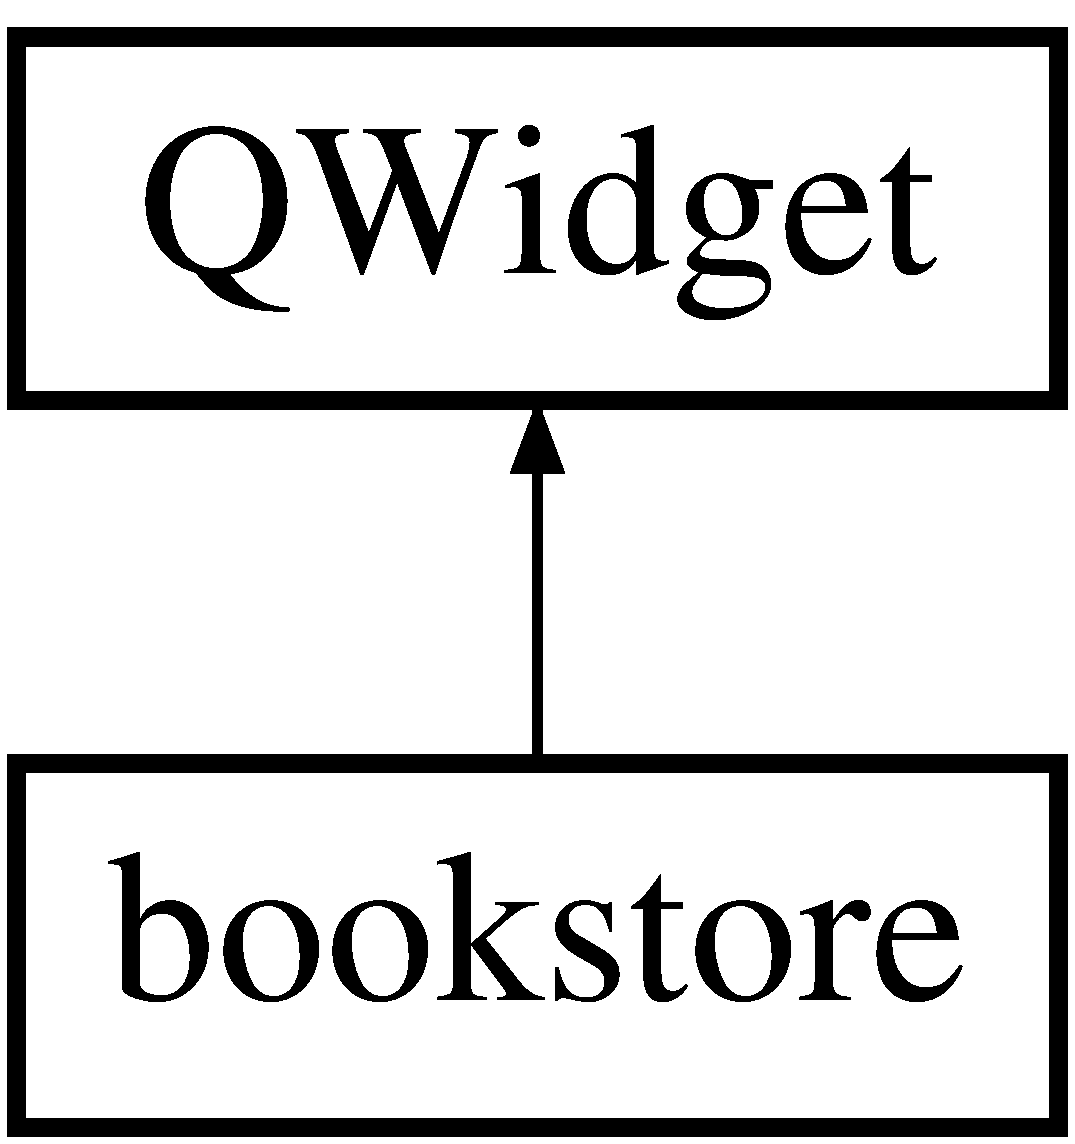
\includegraphics[height=2.000000cm]{classbookstore}
\end{center}
\end{figure}
\subsection*{Public Member Functions}
\begin{DoxyCompactItemize}
\item 
\hyperlink{classbookstore_a57463d718cea231ddafd9012361dff0f}{bookstore} (Q\+Widget $\ast$parent=0)
\end{DoxyCompactItemize}


\subsection{Constructor \& Destructor Documentation}
\index{bookstore@{bookstore}!bookstore@{bookstore}}
\index{bookstore@{bookstore}!bookstore@{bookstore}}
\subsubsection[{\texorpdfstring{bookstore(\+Q\+Widget $\ast$parent=0)}{bookstore(QWidget *parent=0)}}]{\setlength{\rightskip}{0pt plus 5cm}bookstore\+::bookstore (
\begin{DoxyParamCaption}
\item[{Q\+Widget $\ast$}]{parent = {\ttfamily 0}}
\end{DoxyParamCaption}
)\hspace{0.3cm}{\ttfamily [explicit]}}\hypertarget{classbookstore_a57463d718cea231ddafd9012361dff0f}{}\label{classbookstore_a57463d718cea231ddafd9012361dff0f}

\begin{DoxyParams}{Parameters}
{\em parent} & \\
\hline
\end{DoxyParams}


The documentation for this class was generated from the following files\+:\begin{DoxyCompactItemize}
\item 
bookstore.\+h\item 
bookstore.\+cpp\end{DoxyCompactItemize}

\hypertarget{classhtmlreader}{}\section{htmlreader Class Reference}
\label{classhtmlreader}\index{htmlreader@{htmlreader}}


The documentation for this class was generated from the following files\+:\begin{DoxyCompactItemize}
\item 
htmlreader.\+h\item 
htmlreader.\+cpp\end{DoxyCompactItemize}

\hypertarget{classjson_parser}{}\section{json\+Parser Class Reference}
\label{classjson_parser}\index{json\+Parser@{json\+Parser}}
\subsection*{Public Member Functions}
\begin{DoxyCompactItemize}
\item 
void \hyperlink{classjson_parser_a47ac594c4d278f477896a5dd894bcda5}{load} (Q\+String file\+Name)
\item 
void \hyperlink{classjson_parser_a61e314ec1b2c1dee7b53015247e8d226}{write} (Q\+String file\+Name)
\end{DoxyCompactItemize}


\subsection{Member Function Documentation}
\index{json\+Parser@{json\+Parser}!load@{load}}
\index{load@{load}!json\+Parser@{json\+Parser}}
\subsubsection[{\texorpdfstring{load(\+Q\+String file\+Name)}{load(QString fileName)}}]{\setlength{\rightskip}{0pt plus 5cm}void json\+Parser\+::load (
\begin{DoxyParamCaption}
\item[{Q\+String}]{file\+Name}
\end{DoxyParamCaption}
)}\hypertarget{classjson_parser_a47ac594c4d278f477896a5dd894bcda5}{}\label{classjson_parser_a47ac594c4d278f477896a5dd894bcda5}

\begin{DoxyParams}{Parameters}
{\em file\+Name} & \\
\hline
\end{DoxyParams}
\index{json\+Parser@{json\+Parser}!write@{write}}
\index{write@{write}!json\+Parser@{json\+Parser}}
\subsubsection[{\texorpdfstring{write(\+Q\+String file\+Name)}{write(QString fileName)}}]{\setlength{\rightskip}{0pt plus 5cm}void json\+Parser\+::write (
\begin{DoxyParamCaption}
\item[{Q\+String}]{file\+Name}
\end{DoxyParamCaption}
)}\hypertarget{classjson_parser_a61e314ec1b2c1dee7b53015247e8d226}{}\label{classjson_parser_a61e314ec1b2c1dee7b53015247e8d226}

\begin{DoxyParams}{Parameters}
{\em file\+Name} & \\
\hline
\end{DoxyParams}


The documentation for this class was generated from the following files\+:\begin{DoxyCompactItemize}
\item 
jsonparser.\+h\item 
jsonparser.\+cpp\end{DoxyCompactItemize}

\hypertarget{class_libary}{}\section{Libary Class Reference}
\label{class_libary}\index{Libary@{Libary}}


The documentation for this class was generated from the following files\+:\begin{DoxyCompactItemize}
\item 
library.\+h\item 
library.\+cpp\end{DoxyCompactItemize}

\hypertarget{classlogin_dialog}{}\section{login\+Dialog Class Reference}
\label{classlogin_dialog}\index{login\+Dialog@{login\+Dialog}}
Inheritance diagram for login\+Dialog\+:\begin{figure}[H]
\begin{center}
\leavevmode
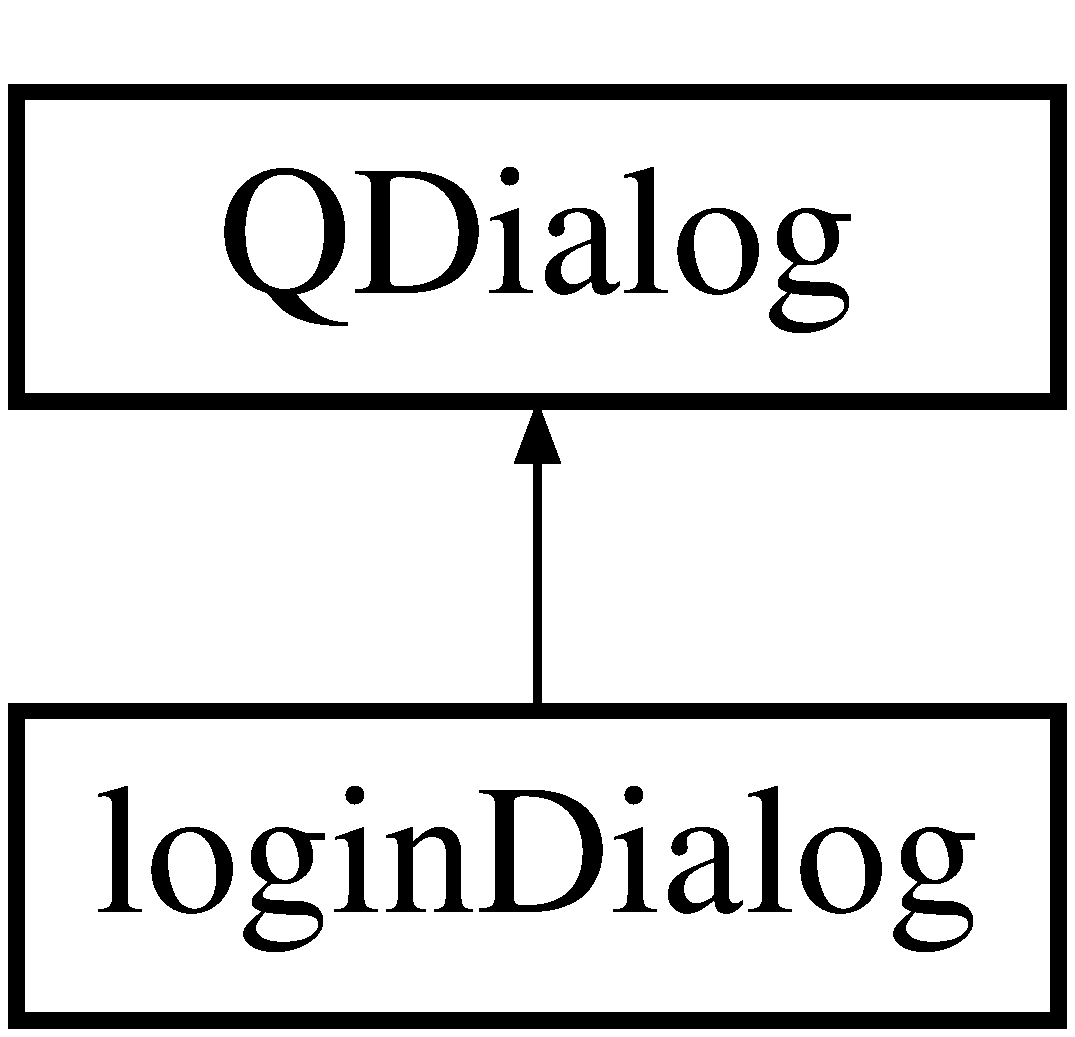
\includegraphics[height=2.000000cm]{classlogin_dialog}
\end{center}
\end{figure}
\subsection*{Public Member Functions}
\begin{DoxyCompactItemize}
\item 
\hyperlink{classlogin_dialog_a69d4c0f180ab04f7891b9a01cdfda8fa}{login\+Dialog} (Q\+Widget $\ast$parent)
\end{DoxyCompactItemize}


\subsection{Constructor \& Destructor Documentation}
\index{login\+Dialog@{login\+Dialog}!login\+Dialog@{login\+Dialog}}
\index{login\+Dialog@{login\+Dialog}!login\+Dialog@{login\+Dialog}}
\subsubsection[{\texorpdfstring{login\+Dialog(\+Q\+Widget $\ast$parent)}{loginDialog(QWidget *parent)}}]{\setlength{\rightskip}{0pt plus 5cm}login\+Dialog\+::login\+Dialog (
\begin{DoxyParamCaption}
\item[{Q\+Widget $\ast$}]{parent}
\end{DoxyParamCaption}
)\hspace{0.3cm}{\ttfamily [explicit]}}\hypertarget{classlogin_dialog_a69d4c0f180ab04f7891b9a01cdfda8fa}{}\label{classlogin_dialog_a69d4c0f180ab04f7891b9a01cdfda8fa}

\begin{DoxyParams}{Parameters}
{\em parent} & \\
\hline
\end{DoxyParams}


The documentation for this class was generated from the following files\+:\begin{DoxyCompactItemize}
\item 
logindialog.\+h\item 
logindialog.\+cpp\end{DoxyCompactItemize}

\hypertarget{class_main_window}{}\section{Main\+Window Class Reference}
\label{class_main_window}\index{Main\+Window@{Main\+Window}}
Inheritance diagram for Main\+Window\+:\begin{figure}[H]
\begin{center}
\leavevmode
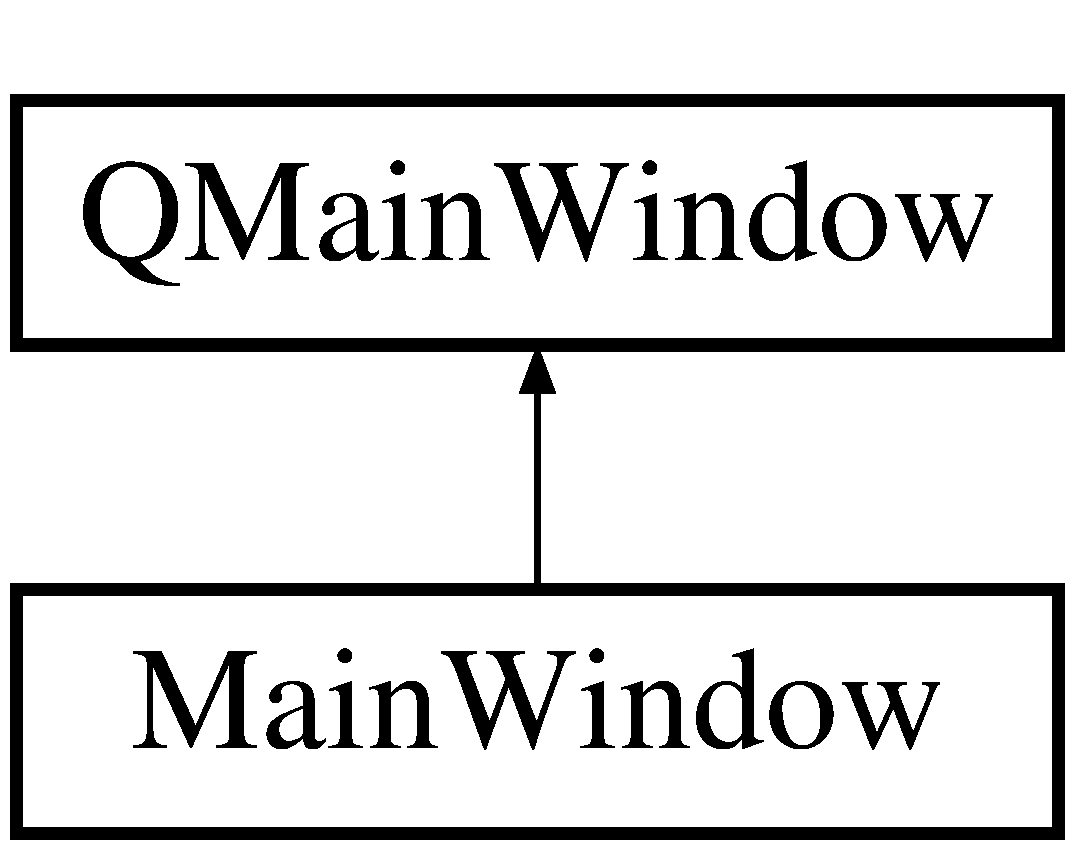
\includegraphics[height=2.000000cm]{class_main_window}
\end{center}
\end{figure}
\subsection*{Public Member Functions}
\begin{DoxyCompactItemize}
\item 
\hyperlink{class_main_window_a8b244be8b7b7db1b08de2a2acb9409db}{Main\+Window} (Q\+Widget $\ast$parent=0)
\begin{DoxyCompactList}\small\item\em \hyperlink{class_main_window_a8b244be8b7b7db1b08de2a2acb9409db}{Main\+Window\+::\+Main\+Window}. \end{DoxyCompactList}\item 
\hyperlink{class_main_window_ae98d00a93bc118200eeef9f9bba1dba7}{$\sim$\+Main\+Window} ()
\begin{DoxyCompactList}\small\item\em \hyperlink{class_main_window_ae98d00a93bc118200eeef9f9bba1dba7}{Main\+Window\+::$\sim$\+Main\+Window}. \end{DoxyCompactList}\item 
void {\bfseries splashscreen} ()\hypertarget{class_main_window_a6d788add1549fb237ef3a9e8fa2bd394}{}\label{class_main_window_a6d788add1549fb237ef3a9e8fa2bd394}

\item 
void \hyperlink{class_main_window_a2e88bd3ea5604f4b4a4056ab4de369d4}{load\+File} (Q\+String file\+Name)
\begin{DoxyCompactList}\small\item\em \hyperlink{class_main_window_a2e88bd3ea5604f4b4a4056ab4de369d4}{Main\+Window\+::load\+File}. \end{DoxyCompactList}\end{DoxyCompactItemize}


\subsection{Constructor \& Destructor Documentation}
\index{Main\+Window@{Main\+Window}!Main\+Window@{Main\+Window}}
\index{Main\+Window@{Main\+Window}!Main\+Window@{Main\+Window}}
\subsubsection[{\texorpdfstring{Main\+Window(\+Q\+Widget $\ast$parent=0)}{MainWindow(QWidget *parent=0)}}]{\setlength{\rightskip}{0pt plus 5cm}Main\+Window\+::\+Main\+Window (
\begin{DoxyParamCaption}
\item[{Q\+Widget $\ast$}]{parent = {\ttfamily 0}}
\end{DoxyParamCaption}
)\hspace{0.3cm}{\ttfamily [explicit]}}\hypertarget{class_main_window_a8b244be8b7b7db1b08de2a2acb9409db}{}\label{class_main_window_a8b244be8b7b7db1b08de2a2acb9409db}


\hyperlink{class_main_window_a8b244be8b7b7db1b08de2a2acb9409db}{Main\+Window\+::\+Main\+Window}. 


\begin{DoxyParams}{Parameters}
{\em parent} & construtor \\
\hline
{\em parent} & \\
\hline
\end{DoxyParams}
\index{Main\+Window@{Main\+Window}!````~Main\+Window@{$\sim$\+Main\+Window}}
\index{````~Main\+Window@{$\sim$\+Main\+Window}!Main\+Window@{Main\+Window}}
\subsubsection[{\texorpdfstring{$\sim$\+Main\+Window()}{~MainWindow()}}]{\setlength{\rightskip}{0pt plus 5cm}Main\+Window\+::$\sim$\+Main\+Window (
\begin{DoxyParamCaption}
{}
\end{DoxyParamCaption}
)}\hypertarget{class_main_window_ae98d00a93bc118200eeef9f9bba1dba7}{}\label{class_main_window_ae98d00a93bc118200eeef9f9bba1dba7}


\hyperlink{class_main_window_ae98d00a93bc118200eeef9f9bba1dba7}{Main\+Window\+::$\sim$\+Main\+Window}. 

destructor 

\subsection{Member Function Documentation}
\index{Main\+Window@{Main\+Window}!load\+File@{load\+File}}
\index{load\+File@{load\+File}!Main\+Window@{Main\+Window}}
\subsubsection[{\texorpdfstring{load\+File(\+Q\+String file\+Name)}{loadFile(QString fileName)}}]{\setlength{\rightskip}{0pt plus 5cm}void Main\+Window\+::load\+File (
\begin{DoxyParamCaption}
\item[{Q\+String}]{file\+Name}
\end{DoxyParamCaption}
)}\hypertarget{class_main_window_a2e88bd3ea5604f4b4a4056ab4de369d4}{}\label{class_main_window_a2e88bd3ea5604f4b4a4056ab4de369d4}


\hyperlink{class_main_window_a2e88bd3ea5604f4b4a4056ab4de369d4}{Main\+Window\+::load\+File}. 


\begin{DoxyParams}{Parameters}
{\em file\+Name} & loads a file \\
\hline
{\em file\+Name} & \\
\hline
\end{DoxyParams}


The documentation for this class was generated from the following files\+:\begin{DoxyCompactItemize}
\item 
mainwindow.\+h\item 
mainwindow.\+cpp\end{DoxyCompactItemize}

\hypertarget{classpdf_reader}{}\section{pdf\+Reader Class Reference}
\label{classpdf_reader}\index{pdf\+Reader@{pdf\+Reader}}
\subsection*{Static Public Member Functions}
\begin{DoxyCompactItemize}
\item 
static Q\+Image \hyperlink{classpdf_reader_a475f289a1ff8670e25592d1f00bcdc1e}{load} (Q\+String)
\item 
static Q\+String \hyperlink{classpdf_reader_adadd3f2612352a9d62434f3cb447f96b}{search} (Q\+String value)
\end{DoxyCompactItemize}


\subsection{Member Function Documentation}
\index{pdf\+Reader@{pdf\+Reader}!load@{load}}
\index{load@{load}!pdf\+Reader@{pdf\+Reader}}
\subsubsection[{\texorpdfstring{load(\+Q\+String)}{load(QString)}}]{\setlength{\rightskip}{0pt plus 5cm}Q\+Image pdf\+Reader\+::load (
\begin{DoxyParamCaption}
\item[{Q\+String}]{file\+Name}
\end{DoxyParamCaption}
)\hspace{0.3cm}{\ttfamily [static]}}\hypertarget{classpdf_reader_a475f289a1ff8670e25592d1f00bcdc1e}{}\label{classpdf_reader_a475f289a1ff8670e25592d1f00bcdc1e}

\begin{DoxyParams}{Parameters}
{\em Q\+String} & \\
\hline
\end{DoxyParams}
\begin{DoxyReturn}{Returns}
Q\+Image 
\end{DoxyReturn}
\index{pdf\+Reader@{pdf\+Reader}!search@{search}}
\index{search@{search}!pdf\+Reader@{pdf\+Reader}}
\subsubsection[{\texorpdfstring{search(\+Q\+String value)}{search(QString value)}}]{\setlength{\rightskip}{0pt plus 5cm}static Q\+String pdf\+Reader\+::search (
\begin{DoxyParamCaption}
\item[{Q\+String}]{value}
\end{DoxyParamCaption}
)\hspace{0.3cm}{\ttfamily [static]}}\hypertarget{classpdf_reader_adadd3f2612352a9d62434f3cb447f96b}{}\label{classpdf_reader_adadd3f2612352a9d62434f3cb447f96b}

\begin{DoxyParams}{Parameters}
{\em value} & \\
\hline
\end{DoxyParams}
\begin{DoxyReturn}{Returns}
Q\+String 
\end{DoxyReturn}


The documentation for this class was generated from the following files\+:\begin{DoxyCompactItemize}
\item 
pdfreader.\+h\item 
pdfreader.\+cpp\end{DoxyCompactItemize}

\hypertarget{classsettingsdialog}{}\section{settingsdialog Class Reference}
\label{classsettingsdialog}\index{settingsdialog@{settingsdialog}}
Inheritance diagram for settingsdialog\+:\begin{figure}[H]
\begin{center}
\leavevmode
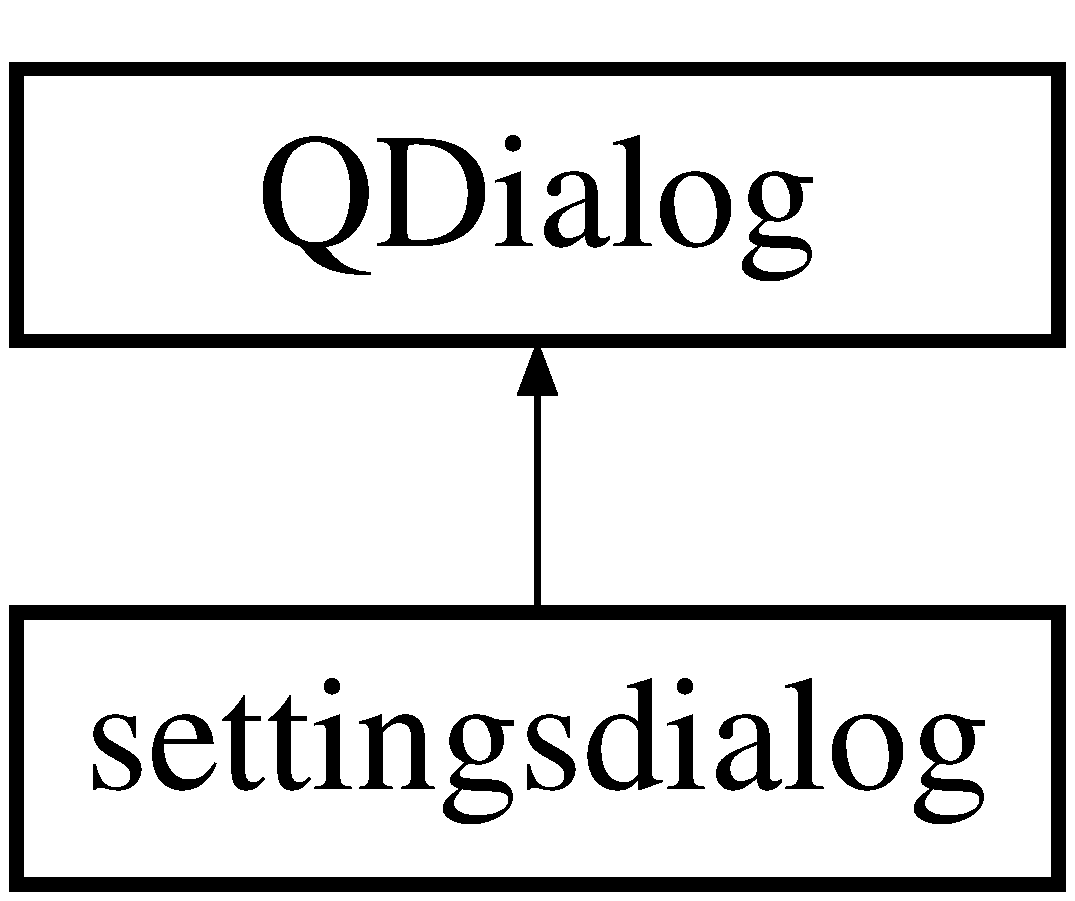
\includegraphics[height=2.000000cm]{classsettingsdialog}
\end{center}
\end{figure}
\subsection*{Public Member Functions}
\begin{DoxyCompactItemize}
\item 
\hyperlink{classsettingsdialog_a519e6f51ccf571de1cb017421760c7a0}{settingsdialog} (Q\+Widget $\ast$parent)
\end{DoxyCompactItemize}


\subsection{Constructor \& Destructor Documentation}
\index{settingsdialog@{settingsdialog}!settingsdialog@{settingsdialog}}
\index{settingsdialog@{settingsdialog}!settingsdialog@{settingsdialog}}
\subsubsection[{\texorpdfstring{settingsdialog(\+Q\+Widget $\ast$parent)}{settingsdialog(QWidget *parent)}}]{\setlength{\rightskip}{0pt plus 5cm}settingsdialog\+::settingsdialog (
\begin{DoxyParamCaption}
\item[{Q\+Widget $\ast$}]{parent}
\end{DoxyParamCaption}
)\hspace{0.3cm}{\ttfamily [explicit]}}\hypertarget{classsettingsdialog_a519e6f51ccf571de1cb017421760c7a0}{}\label{classsettingsdialog_a519e6f51ccf571de1cb017421760c7a0}

\begin{DoxyParams}{Parameters}
{\em parent} & \\
\hline
\end{DoxyParams}


The documentation for this class was generated from the following files\+:\begin{DoxyCompactItemize}
\item 
settingsdialog.\+h\item 
settingsdialog.\+cpp\end{DoxyCompactItemize}

\hypertarget{classtxteditor}{}\section{txteditor Class Reference}
\label{classtxteditor}\index{txteditor@{txteditor}}
\subsection*{Public Member Functions}
\begin{DoxyCompactItemize}
\item 
Q\+String \hyperlink{classtxteditor_a526aaa5199548d8dabc0bbab5f09f9d3}{read} (Q\+String file\+Name)
\item 
bool \hyperlink{classtxteditor_a075c5b3c3ae3eda6480f46183cb6afcf}{write} ()
\item 
void \hyperlink{classtxteditor_a0bf6db11b2d59f05d37fc24d38f8faa2}{display} (Q\+String string)
\end{DoxyCompactItemize}


\subsection{Member Function Documentation}
\index{txteditor@{txteditor}!display@{display}}
\index{display@{display}!txteditor@{txteditor}}
\subsubsection[{\texorpdfstring{display(\+Q\+String string)}{display(QString string)}}]{\setlength{\rightskip}{0pt plus 5cm}void txteditor\+::display (
\begin{DoxyParamCaption}
\item[{Q\+String}]{string}
\end{DoxyParamCaption}
)}\hypertarget{classtxteditor_a0bf6db11b2d59f05d37fc24d38f8faa2}{}\label{classtxteditor_a0bf6db11b2d59f05d37fc24d38f8faa2}

\begin{DoxyParams}{Parameters}
{\em string} & \\
\hline
\end{DoxyParams}
\index{txteditor@{txteditor}!read@{read}}
\index{read@{read}!txteditor@{txteditor}}
\subsubsection[{\texorpdfstring{read(\+Q\+String file\+Name)}{read(QString fileName)}}]{\setlength{\rightskip}{0pt plus 5cm}Q\+String txteditor\+::read (
\begin{DoxyParamCaption}
\item[{Q\+String}]{file\+Name}
\end{DoxyParamCaption}
)}\hypertarget{classtxteditor_a526aaa5199548d8dabc0bbab5f09f9d3}{}\label{classtxteditor_a526aaa5199548d8dabc0bbab5f09f9d3}

\begin{DoxyParams}{Parameters}
{\em file\+Name} & \\
\hline
\end{DoxyParams}
\begin{DoxyReturn}{Returns}
Q\+String 
\end{DoxyReturn}
\index{txteditor@{txteditor}!write@{write}}
\index{write@{write}!txteditor@{txteditor}}
\subsubsection[{\texorpdfstring{write()}{write()}}]{\setlength{\rightskip}{0pt plus 5cm}bool txteditor\+::write (
\begin{DoxyParamCaption}
{}
\end{DoxyParamCaption}
)}\hypertarget{classtxteditor_a075c5b3c3ae3eda6480f46183cb6afcf}{}\label{classtxteditor_a075c5b3c3ae3eda6480f46183cb6afcf}
\begin{DoxyReturn}{Returns}
bool 
\end{DoxyReturn}


The documentation for this class was generated from the following files\+:\begin{DoxyCompactItemize}
\item 
txteditor.\+h\item 
txteditor.\+cpp\end{DoxyCompactItemize}

\hypertarget{classxml_reader}{}\section{xml\+Reader Class Reference}
\label{classxml_reader}\index{xml\+Reader@{xml\+Reader}}
\subsection*{Public Member Functions}
\begin{DoxyCompactItemize}
\item 
Q\+String \hyperlink{classxml_reader_abd4bd8e199edefdf98cf853dce90d748}{load} (Q\+String file\+Name)
\item 
Q\+String \hyperlink{classxml_reader_a29c2e12cf679bc608cf51b56cf20b38e}{load\+Info} (Q\+String file\+Name)
\item 
bool \hyperlink{classxml_reader_ad410030cd6771f4a711ac7161dd7fa14}{validate} (Q\+String file\+Name)
\item 
Q\+String\+List \hyperlink{classxml_reader_a2a18ef3e28a17e9c490e49f4017e87a6}{read\+Chapter\+Verses} (Q\+String file\+Name)
\item 
Q\+String \hyperlink{classxml_reader_a0b117509f1a43fefd5557704a2add047}{read\+Book\+Title} (Q\+String file\+Name)
\end{DoxyCompactItemize}


\subsection{Member Function Documentation}
\index{xml\+Reader@{xml\+Reader}!load@{load}}
\index{load@{load}!xml\+Reader@{xml\+Reader}}
\subsubsection[{\texorpdfstring{load(\+Q\+String file\+Name)}{load(QString fileName)}}]{\setlength{\rightskip}{0pt plus 5cm}Q\+String xml\+Reader\+::load (
\begin{DoxyParamCaption}
\item[{Q\+String}]{file\+Name}
\end{DoxyParamCaption}
)}\hypertarget{classxml_reader_abd4bd8e199edefdf98cf853dce90d748}{}\label{classxml_reader_abd4bd8e199edefdf98cf853dce90d748}

\begin{DoxyParams}{Parameters}
{\em file\+Name} & \\
\hline
\end{DoxyParams}
\begin{DoxyReturn}{Returns}
Q\+String 
\end{DoxyReturn}
\index{xml\+Reader@{xml\+Reader}!load\+Info@{load\+Info}}
\index{load\+Info@{load\+Info}!xml\+Reader@{xml\+Reader}}
\subsubsection[{\texorpdfstring{load\+Info(\+Q\+String file\+Name)}{loadInfo(QString fileName)}}]{\setlength{\rightskip}{0pt plus 5cm}Q\+String xml\+Reader\+::load\+Info (
\begin{DoxyParamCaption}
\item[{Q\+String}]{file\+Name}
\end{DoxyParamCaption}
)}\hypertarget{classxml_reader_a29c2e12cf679bc608cf51b56cf20b38e}{}\label{classxml_reader_a29c2e12cf679bc608cf51b56cf20b38e}

\begin{DoxyParams}{Parameters}
{\em file\+Name} & \\
\hline
\end{DoxyParams}
\begin{DoxyReturn}{Returns}
Q\+String 
\end{DoxyReturn}
\index{xml\+Reader@{xml\+Reader}!read\+Book\+Title@{read\+Book\+Title}}
\index{read\+Book\+Title@{read\+Book\+Title}!xml\+Reader@{xml\+Reader}}
\subsubsection[{\texorpdfstring{read\+Book\+Title(\+Q\+String file\+Name)}{readBookTitle(QString fileName)}}]{\setlength{\rightskip}{0pt plus 5cm}Q\+String xml\+Reader\+::read\+Book\+Title (
\begin{DoxyParamCaption}
\item[{Q\+String}]{file\+Name}
\end{DoxyParamCaption}
)}\hypertarget{classxml_reader_a0b117509f1a43fefd5557704a2add047}{}\label{classxml_reader_a0b117509f1a43fefd5557704a2add047}

\begin{DoxyParams}{Parameters}
{\em file\+Name} & \\
\hline
\end{DoxyParams}
\begin{DoxyReturn}{Returns}
Q\+String 
\end{DoxyReturn}
\index{xml\+Reader@{xml\+Reader}!read\+Chapter\+Verses@{read\+Chapter\+Verses}}
\index{read\+Chapter\+Verses@{read\+Chapter\+Verses}!xml\+Reader@{xml\+Reader}}
\subsubsection[{\texorpdfstring{read\+Chapter\+Verses(\+Q\+String file\+Name)}{readChapterVerses(QString fileName)}}]{\setlength{\rightskip}{0pt plus 5cm}Q\+String\+List xml\+Reader\+::read\+Chapter\+Verses (
\begin{DoxyParamCaption}
\item[{Q\+String}]{file\+Name}
\end{DoxyParamCaption}
)}\hypertarget{classxml_reader_a2a18ef3e28a17e9c490e49f4017e87a6}{}\label{classxml_reader_a2a18ef3e28a17e9c490e49f4017e87a6}

\begin{DoxyParams}{Parameters}
{\em file\+Name} & \\
\hline
\end{DoxyParams}
\begin{DoxyReturn}{Returns}
Q\+String\+List 
\end{DoxyReturn}
\index{xml\+Reader@{xml\+Reader}!validate@{validate}}
\index{validate@{validate}!xml\+Reader@{xml\+Reader}}
\subsubsection[{\texorpdfstring{validate(\+Q\+String file\+Name)}{validate(QString fileName)}}]{\setlength{\rightskip}{0pt plus 5cm}bool xml\+Reader\+::validate (
\begin{DoxyParamCaption}
\item[{Q\+String}]{file\+Name}
\end{DoxyParamCaption}
)}\hypertarget{classxml_reader_ad410030cd6771f4a711ac7161dd7fa14}{}\label{classxml_reader_ad410030cd6771f4a711ac7161dd7fa14}

\begin{DoxyParams}{Parameters}
{\em file\+Name} & \\
\hline
\end{DoxyParams}
\begin{DoxyReturn}{Returns}
bool 
\end{DoxyReturn}


The documentation for this class was generated from the following files\+:\begin{DoxyCompactItemize}
\item 
xmlreader.\+h\item 
xmlreader.\+cpp\end{DoxyCompactItemize}

%--- End generated contents ---

% Index
\backmatter
\newpage
\phantomsection
\clearemptydoublepage
\addcontentsline{toc}{chapter}{Index}
\printindex

\end{document}
